\chapter{Concept Art (1961)}

Concept art is first of all an art of which the material is concepts, as the 
material of e.g. music is sound. Since concepts are closely bound up with 
language, concept art is a kind of art of which the material is language. That 
is, unlike e.g.\ a work of music, in which the music proper (as opposed to 
notation, analysis, etc.) is just sound, concept art proper will involve 
language. From the philosophy of language, we learn that a concept may as 
well be thought of as the intension of a name; this is the relation between 
concepts and language.\footnote{The extension of the word 'table' is all 
existing tables; the intension of 'table' is all possible instances of a table.}
The notion of a concept is a vestige of the notion of 
a platonic form (the thing which e.g.\ all tables have in common: tableness), 
which notion is replaced by the notion of a name objectively, metaphysically 
related to its intension (so that all tables now have in common their 
objective relation to table). Now the claim that there can be an objective 
relation between a name and its intension is wrong, and (the word) concept, 
as commonly used now, can be discredited (see \essaytitle{Philosophy 
Proper}). If, however, it is enough for one that there be a subjective relation 
between a name and its intension, namely the unhesitant decision as to the 
way one wants to use the name, the unhesitant decisions to affirm the names 
of some things but not others, then concept is valid language, and concept 
art has a philosophically valid basis. 

Now what is artistic, aesthetic, about a work which is a body of 
concepts? This question can best be answered by telling where concept art 
came from; I developed it in an attempt to straighten out certain traditional 
activities generally regarded as aesthetic. The first of these is structure art, 
music, visual art, etc., in which the important thing is \enquote{structure.} My 
definitive discussion of structure art is in my unpublished\editornote{We provide this for you in the appendix!} essay \essaytitle{Structure 
Art and Pure Mathematics}; here I will just summarize that discussion. Much 
structure art is a vestige of the time when e.g. music was believed to be 
knowledge, a science, which had important things to say in astronomy etc.
Contemporary structure artists, on the other hand, tend to claim the kind of 
cognitive value for their art that conventional contemporary mathematicians 
claim for mathematics. Modern examples of structure art are the fugue and 
total serial music. These examples illustrate the important division of 
structure art into two kinds according to how the structure is appreciated. In 
the case of a fugue, one is aware of its structure in listening to it; one 
imposes relationships, a categorization (hopefully that intended by the 
composer) on the sounds while listening to them, that is, has an (associated) 
artistic structure experience. In the case of total serial music, the structure is 
such that this cannot be done; one just has to read an analysis of the 
music, definition of the relationships. Now there are two things wrong with 
structure art. First, its cognitive pretensions are utterly wrong. Secondly, by 
trying to be music or whatever (which has nothing to do with knowledge), 
and knowledge represented by structure, structure art both fails, is 
completely boring, as music, and doesn't begin to explore the aesthetic 
possibilities structure can have when freed from trying to be music or 
whatever. The first step in straightening out e.g.\ structure music is to stop 
calling it music, and start saying that the sound is used only to carry the 
structure and that the real point is the structure--and then you will see how 
limited, impoverished, the structure is. Incidentally, anyone who says that 
works of structure music do occasionally have musical value just doesn't 
know how good real music (the Goli Dance of the Baoule; Cans on Windows 
by La Monte Young; the contemporary American hit song Sweets for My 
Sweets, by the Drifters) can get. When you make the change, then since 
structures are concepts, you have concept art. Incidentally, there is another, 
less important kind of art which when straightened out becomes concept art: 
art involving play with the concepts of the art such as, in music, the score, 
performer vs. listener, playing a work. The second criticism of structure art 
applies, with the necessary changes, to this art. 

The second main antecedent of structure art is mathematics. This is the 
result of my revolution in mathematics, presented in my \essaytitle{1966 Mathematical 
Studies}; here I will only summarize. The revolution occured first because for 
reasons of taste I wanted to deemphasize discovery in mathematics, 
mathematics as discovering theorems and proofs. I wasn't good at such 
discovery, and it bored me. The first way I thought of to de-emphasize 
discovery came not later than Summer, 1960; it was that since the value of 
pure mathematics is now regarded as aesthetic rather than cognitive, why not 
try to make up aesthetic theorems, without considering whether they are 
true. The second way, which came at about the same time, was to find, as a 
philosopher, that the conventional claim that theorems and proofs are 
discovered is wrong, for the same reason I have already given that 'concept' 
can be discredited. The third way, which came in the fall-winter of 1960, 
was to work in unexplored regions of formalist mathematics. The resulting 
mathematics still had statements, theorems, proofs, but the latter weren't 
discovered in the way they traditionally were. Now exploration of the wider 
possibilities of mathematics as revolutionized by me tends to lead beyond 
what it makes sense to call mathematics; the category of mathematics, a 
vestige of Platonism, is an unnatural, bad one. My work in mathematics leads 
to the new category of concept art, of which straightened out traditional 
mathematics (mathematics as discovery) is an untypical, small but 
intensively developed part. 

I can now return to the question of why concept art is art. Why isn't it an 
absolutely new, or at least a non-artistic, non-aesthetic activity? The answer 
is that the antecedents of concept art are commonly regarded as artistic, 
aesthetic activities; on a deeper level, interesting concepts, concepts 
enjoyable in themselves, especially as they occur in mathematics, are 
commonly said to have beauty. By calling my activity art, therefore, I am 
simply recognizing this common usage, and the origin of the activity in 
structure art and mathematics. However: it is confusing to call things as 
irrelevant as the emotional enjoyment of (real) music, and the intellectual 
enjoyment of concepts, the same kind of enjoyment. Since concept art 
includes almost everything ever said to be music, at least, which is not music 
for the emotions, perhaps it would be better to restrict art to apply to art for 
the emotions, and recognize my activity as an independent, new activity, 
irrelevant to art (and knowledge). 

\section{Concept Art Version of Mathematics System 3/26/61 (6/19/61)}

An element is the adjacent area (with figure \ref{implications} in it) so long as the 
apparent, perceived, ratio of the length of the vertical line to that of the 
horizontal line (the element's associated ratio) does not change. 

A selection sequence is a sequence of elements of which the first is the one 
having the greatest associated ratio, and each of the others has the associated 
ratio next smaller than that of the preceding one. (To decrease the ratio, 
come to see the vertical line as shorter, relative to the horizontal line, one 
might try measuring the lines with a ruler to convince oneself that the 
vertical one is not longer than the other, and then trying to see the lines as 
equal in length; constructing similar figures with a variety of real (measured) 
ratios and practicing judging these ratios; and so forth.) 

[Observe that the order of elements in a selection sequence may not be the 
order in which one sees them.] 

\begin{figure}
	\centering
	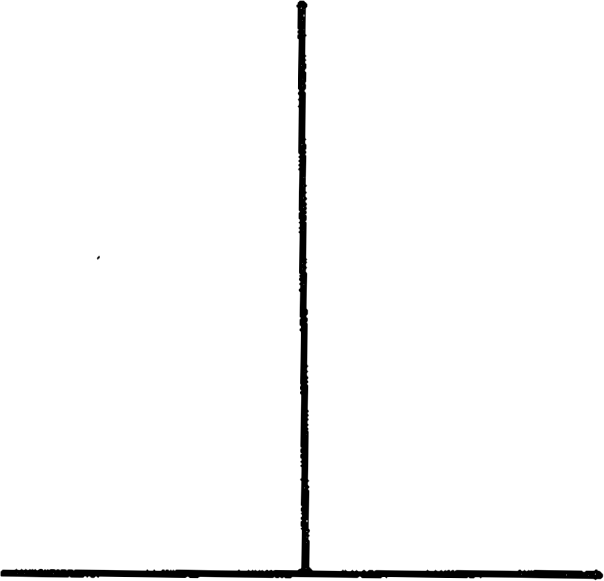
\includegraphics[scale=1]{img/implications}
	\caption{tktk}
	\label{implications}
\end{figure}

\section{Implications---Concept Art Version of Colored Sheet Music No. 1 3/14/61 (10/11/61)}

[This is a mathematical system without general concepts of statement, 
implication, axiom, and proof. Instead, you make the object, and stipulate 
by ostension that it is an axiom, theorem, or whatever. My thesis is that 
since there is no objective relation between name and intension, all 
mathematics is this arbitrary. Originally, the successive statements, or sheets, 
were to be played on an optical audiorecorder.]

\begin{hangers}
The \term{axiom}: a sheet of cheap, thin white typewriter paper.

The axiom implies statement 2 ($S_2$): soak the axiom in inflammable liquid which 
does not leave solid residue when burned; then burn it on horizontal 
rectangular white fireproof surface---$S_2$ is ashes (on surface) 

$S_2$ implies $S_3$: make black and white photograph of $S_2$ in white 
light (image of ashes' rectangle with respect to white surface (that is, of the 
region (of surface, with the ashes on it) with bounding edges parallel to the 
edges of the surface and intersecting the four points in the ashes nearest the 
four edges of the surface) must exactly cover the film); develop film---$S_3$ is 
the negative.

$S_2$ and $S_3$ imply $S_4$: melt $S_4$ and cool in mold to form plastic doubly 
convex lens with small curvature; take color photograph of ashes' rectangle 
in yellow light using this lens; develop film---$S_5$ is color negative.

$S_2$ and $S_4$ imply $S_5$: repeat last step with $S_4$ (instead of $S_3$), using red 
light---$S_5$ is second color negative 

$S_2$ and $S_5$ imply $S_6$: repeat last step with $S_5$, using blue light---$S_6$ is third 
color negative 

$S_2$ and $S_6$ imply $S_7$: make lens from $S_6$ mixed with the ashes which have 
been being photographed; make black and white photograph, in white fight, 
of that part of the white surface where the ashes' rectangle was; develop film 
--- $S_7$ is second black and white negative 

$S_2$, $S_6$, and $S_7$ imply the theorem: melt, mold, and cool lens used in last 
step to form negative, and make lens from $S_7$; using negative and lens in an 
enlarger, make two prints, an enlargement and a reduction--enlargement and 
reduction together constitute the theorem. 
\end{hangers}

\section{Concept Art: \sysname{Innperseqs} (May--July 1961)}

\begin{sysrules}
	A \enquote{h\u{a}lpoint} iff whatever is at any point in space, in the fading rainbow halo 
which appears to surround a small bright light when one looks at it through 
glasses fogged by having been breathed on, for as long as the point is in the 
halo. 

An \enquote{init`point} iff a h\u{a}lpoint in the initial vague outer ring of its halo. 


An \enquote{inn`pers\u{e}q} iff a sequence of sequences of h\u{a}lpoints such that all the 
h\u{a}lpoints are on one (initial) radius of a halo; the members of the first 
sequence are init`points; for each of the other sequences, the first member (a 
consequent) is got from the non-first members of the preceding sequence 
(the antecedents) by being the inner endpoint of the radial segment in the 
vague outer ring when they are on the segment, and the other members (if 
any) are init`points or first members of preceding sequences; all first members 
of sequences other than the last [two] appear as non-first members, and 
h\u{a}lpoints appear only once as non-first members; and the last sequence has 
one member. 
\end{sysrules}

\section{\sysname{Indeterminacy}}

\begin{sysrules}
	A $\ulcorner$totally determinate inn`pers\u{e}q$\urcorner$ iff an inn`pers\u{e}q in which one is aware of 
	(specifies) all h\u{a}lpoints. 

	An $\ulcorner$antecedentally indeterminate inn`pers\u{e}q$\urcorner$ iff an inn`pers\u{e}q in which one is 
aware of (specifies) only each consequent and the radial seqment beyond it. 

	A $\ulcorner$h\u{a}lpointally indeterminate inn`pers\u{e}q$\urcorner$ iff an inn`pers\u{e}q in which one is 
aware of (specifies) only the radial segment in the vague outer ring, and its 
inner endpoint, as it progresses inward. 
\end{sysrules}
